\section{Introduction}
Cluster computing has become widespread, leading to a proliferation of
research on improving performance.  In order to run data-parallel
computations more efficiently and more quickly, researchers have attempted
to tackle a variety of problems that arise in this setting,
including improving
fairness~\cite{zaharia2008improving,hindman2011mesos},
handling preemption~\cite{ananthanarayanan2012true,isard2009quincy},
mitigating stragglers~\cite{ananthanarayanan2010reining,anathanarayanan2012why},
and reducing skew~\cite{ananthanarayanan2011scarlett,kwon2012skewtune,gufler2012load}.
%These efforts have significantly improved performance and efficiency.
We argue that a single variable affects all of these challenges: the
granularity of tasks.
%This paper argues that a single variable affects all of these scheduling
%challenges
%Yet, they have surprisingly not explored a single variable that affects all
%of the
%aforementioned challenges: the granularity of tasks.
Historically, task launch overheads have prevented users from running
short tasks; however, recent improves im distributed file systems and
scheduling have eliminated these scaling bottlenecks.
%prohibited the use of sub-second
%tasks; however, recent advances in scheduler and
Thus, we argue for
breaking all jobs into \emph{tiny tasks}, which alleviates or eliminates
all of the above problems:
%solves many problems in
%current data-parallel frameworks:

\eat{
Computer systems schedule and manage a variety of types of work:
%Today's systems accept work in discrete units:
networks process flows of data
between two endpoints, operating systems execute individual applications, and
data centers process data in individual jobs.  In the context of networks and
operating systems, system designers have found that large, indivisible units of work limit utilization and load balancing,
and complicate fair sharing.  Instead, networks divide large flows into small
packets, and operating systems run applications in pre-emptable units of a
few milliseconds.  This paper argues for
applying a similar model to data centers by breaking all jobs into
``tiny tasks,'' each of which runs for a few hundred
milliseconds. We argue that even batch jobs that take hours to complete
should be broken into tiny units of work that each complete quickly.

Tiny tasks solve two major problems in current data-parallel frameworks:
%Decreased task runtimes solve two major problems in today's datacenters:
}
\vspace{4pt}\noindent\textbf{Batch and interactive sharing:}
Current clusters are forced to tradeoff utilization and responsiveness.
In a highly utilized cluster, if a high priority job arrives, the job may
need to wait for long-running tasks to complete before being launched.
On the other end of the spectrum, a cluster can maintain a reserved
set of machines for high priority jobs, which provides responsiveness at
the expense of utilization.
%a high priority job in a highly utilized cluster might
%need to wait for long-running tasks to complete before being run.
However, tiny tasks allow a cluster to be \emph{both} responsive and highly utilized, since small tasks ensure frequent opportunities for new,
higher priority jobs to be launched.
\eat{
Long task runtimes make it challenging to run both batch and interactive
jobs on the same cluster. In particular, task lengths place a lower bound on
the time before resources allocated to a running task can be recovered. A new
task therefore must wait for running tasks to finish before it can start running.
This waiting time is a significant contributor to task latency, and thus adversly
affects the request latency for interactive jobs.

One must tradeoff between
cluster utilization and responsiveness, limiting the benefits of sharing
a cluster. By reducing task runtimes to an acceptably small value, tiny
tasks allow batch and interactive jobs share the same resources, without
trading off request latency.
}

\vspace{4pt}\noindent\textbf{Straggler mitigation:}
Prior work has shown that job runtimes are largely determined by
stragglers: tasks that take much longer to complete than other tasks in the
job. This problem has led to a wide variety of techniques to ensure that
work is evenly balanced across tasks, and to speculatively launch
redundant tasks when a task appears to be running on a slow machine.
Tiny tasks eliminate the straggler problem because work is allocated to
machines at fine granularity, so work will automatically be evenly spread
over available resources, and slower machines will automatically be assigned
less work. Preliminary simulations and evaluation using Spark demonstrate
that by eliminating the straggler problem, tiny tasks can improve response
times by a factor of \fixme{5}.
\eat{
Prior work has shown that tasks runtimes exhibit a long
tailed distribution, and are highly variable. This variance can be caused by
a number of factors, including slow machines, congested networks, a single task
processing larger amount of data, or a combination of the above.
Many mechanisms have been suggested for mitigating
the effects of this variability, generally either by avoiding causes of these
long task runtimes, or by speculatively launching additional tasks in response to slow tasks.
By providing the scheduler with fine grained control over job execution, tiny
tasks makes such mitigation easier, allowing the scheduler to change the resources
allocated to a job in response to outliers.\\
}


Using smaller task durations offers performance improvements even in
today's frameworks.  However, we propose task durations of at most
hundreds of milliseconds, which cannot be fully supported without addressing
numerous challenges. First, small tasks require a highly scalable scheduler
that can make frequent scheduling decisions. Second,
task launch overheads must be small enough so as not to counteract the
benefits from using small tasks.
Third, tiny tasks must operate on correspondingly tiny amounts
of data, which requires a file system that can handle a large number of tiny
file blocks. Finally, tiny tasks require modifications to current programming
models to allow \emph{all} jobs to be split into tiny tasks. We propose a system
that addresses these challenges using a distributed scheduler, a distributed
file system, and a pipelined execution model. Our proposed system supports
100 microsecond task launches, and allows most applications to be
expressed in terms of a set of tiny tasks.

This paper begins by quantifying the benefits of tiny tasks in~\S\ref{sec:benefits}.
We present a preliminary system design that addresses the challenges of
supporting tiny tasks in~\S\ref{sec:architecture},
and explore design alternatives and related work in~\S\ref{sec:alternate}.
\eat{
Existing data-parallel systems have engineering limitations in their distributed
file systems and cluster schedulers that prevent short task runtimes. For example, in
large Hadoop clusters, a larger block size is advised to avoid overflowing the name node.
Hadoop also piggybacks the heartbeat messages to send scheduling decisions, which
results in high scheduling latency.
Current frameworks need to be re-architected to enable tasks to be broken into even smaller
units.
Recent work on distributed filesystems\cite{nightingale2012flat} and cluster
schedulers\cite{ousterhoutbatch} present the first steps towards
building a cluster framework that allows for tiny tasks. While these new filesystems
and schedulers address the scalability problems, many challenges remain. In particular,
efficient use of tiny tasks requires that the overhead for launching a task is small. Current
frameworks take on the order of several hundred milliseconds to a second to launch a task, negating
many of the gains provided by a system with sub-second task lengths. Similarly, any system
supporting tiny tasks must provide additional architectural support for more easily dividing tasks.
}
\begin{figure*}[!ht]
  \centering
  \vspace{-0.2in}
  \begin{minipage}[t]{0.45\textwidth}
    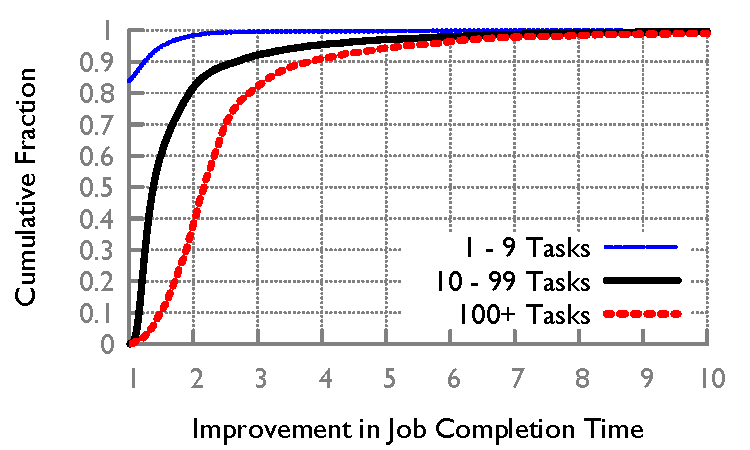
\includegraphics[width=\textwidth]{figures/binpacked1-sep}
    \vspace{-4ex}
    \caption{ Improvement from perfectly balancing the total machine time for the job across tasks. }
    \label{fig:binpacked}
  \end{minipage}
  \hspace{1.2em}
  \begin{minipage}[t]{0.45\textwidth}
    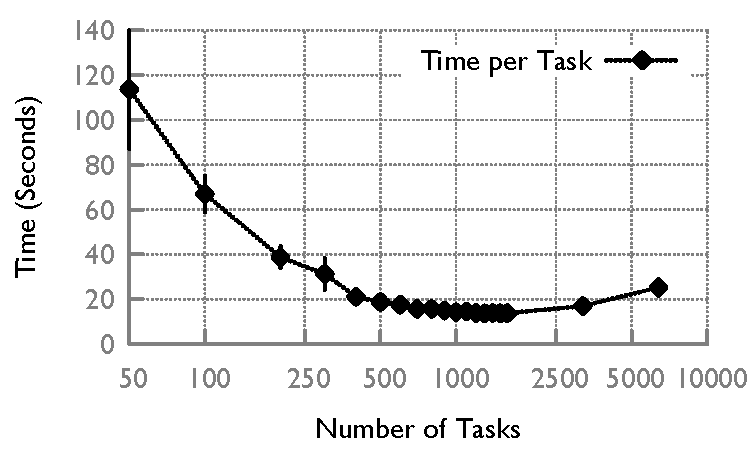
\includegraphics[width=\textwidth]{figures/spark-skew-results}
    \vspace{-4ex}
    \caption{Improvement from using tiny tasks in a cluster where 20\% of machines
take 21x longer to run each task. Error bars depict standard deviation.}
    \label{fig:sparkskew}
  \end{minipage}
  \hspace{.5em}
\end{figure*}
